% Copyright 2005-2016 Airbus-EDF-IMACS-Phimeca
% Permission is granted to copy, distribute and/or modify this document
% under the terms of the GNU Free Documentation License, Version 1.2
% or any later version published by the Free Software Foundation;
% with no Invariant Sections, no Front-Cover Texts, and no Back-Cover
% Texts.  A copy of the license is included in the section entitled "GNU
% Free Documentation License".
\renewcommand{\filename}{docUC_InputNoData_Mixture.tex}
\renewcommand{\filetitle}{UC : Creation  of a nD distribution from a Mixture}

% \HeaderNNIILevel
% \HeaderIILevel
\HeaderIIILevel

\label{Mixture}

\index{Distribution!Mixture}
\index{Graph!PDF-CDF curves}
\index{Graph Manipulation!Bounding box}
\index{Graph Manipulation!View}
\index{Graph Manipulation!Show}

In OpenTURNS, a Mixture is a distribution which probability density function is a linear combination of probability density functions.\\

The objective of this Use Case is to model a distribution, defined as a mixture :
\begin {equation}\label{mixPDF}
  p(\vect{x}) = \sum_{i=1}^{n} a_i p_i(\vect{x})
\end{equation}
where
\begin {equation}\label{mixcons}
  \sum_{i=1}^{n} a_i = 1
\end{equation}
and
\begin {equation}\label{mixcons2}
  \forall i,  \, a_i \geq 0
\end{equation}

OpenTURNS automatically normalizes the  weights so the User can give $a_i$ which don't verify the constraint (\ref{mixcons}). \\
By default, the weights are taken equal to $\frac{1}{n}$.\\

The example here is a mixture of three univariate distributions: Triangular(1.0, 2.0, 4.0), Normal(-1.0, 1.0) and Uniform(5.0, 6.0), with respective weights : (0.2, 0.3, 0.5).\\
The PDF and CDF graphs the mixture distribution are drawn in Figures \ref{mixtureGraphPDF} and  \ref{mixtureGraphCDF}.\\

Note that it is possible to create a mixture of copula. The result still remains a copula.

\textspace\\
\noindent%
\requirements{
  \begin{description}
  \item[$\bullet$] some distributions : {\itshape dist1, dist2}
  \item[type:] Distribution
  \item[$\bullet$] some  copulas: {\itshape cop1, cop2}
  \item[type:] Distribution
  \end{description}
}
             {
               \begin{description}
               \item[$\bullet$] a mixture distribution : {\itshape myMixtDist}
               \item[type:] Mixture
               \item[$\bullet$] a mixture copula : {\itshape myMixtCop}
               \item[type:] Mixture
               \end{description}
             }

             \textspace\\
             Python script for this UseCase :

             \inputscript{script_docUC_InputNoData_Mixture}

             \textspace\\


             \begin{figure}[H]
               \begin{center}
                 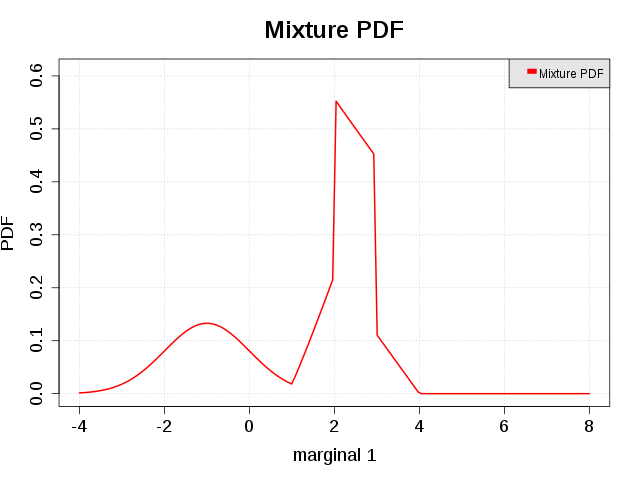
\includegraphics[width=10cm]{Figures/pdf_Mixture.png}
                 \caption{PDF of the Mixture distribution = 0.2*Triangular(1.0, 2.0, 4.0) + 0.5*Normal(-1.0, 1.0) + 0.3*Uniform(5.0, 6.0)}
                 \label{mixtureGraphPDF}
               \end{center}
             \end{figure}

             \begin{figure}[H]
               \begin{center}
                 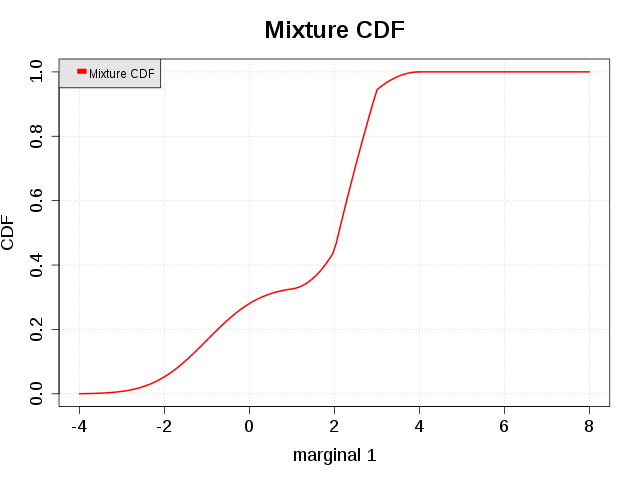
\includegraphics[width=10cm]{Figures/cdf_Mixture.png}
                 \caption{CDF of the Mixture distribution = 0.2*Triangular(1.0, 2.0, 4.0) + 0.5*Normal(-1.0, 1.0) + 0.3*Uniform(5.0, 6.0)}
                 \label{mixtureGraphCDF}
               \end{center}
             \end{figure}
